% Copyright 2026 Sreeram Anil
% SPDX-License-Identifier: CC-BY-4.0
% =============================================================================
%  Fading-memory (exponentially weighted) extended Kalman filter
% =============================================================================
\chapter{Fading-memory extended Kalman filter (Fading-EKF)}
\label{ch:fadingekf}

\section*{At a glance}
\begin{tabular}{@{}l>{\raggedright\arraybackslash}p{0.76\textwidth}@{}}
Family & Adaptive Kalman \\
Header & \texttt{include/estkit/filters/fading\_kf.hpp} \\
Registered name & \texttt{Fading-EKF} \\
State dimension & $n_x = 4$ (cell model) --- generic in $n_x, n_u, n_y$ \\
Cost per step & EKF $+\,n_x^2$ multiplies $+\,\mathcal{O}(n_x^2)$ clamp; $\approx 500$\,ns/step, no heap \\
Primary references & \cite{sorenson1971fading,simon2006,andersonmoore1979,jazwinski1970} \\
\end{tabular}

\section{Motivation and aerospace/BMS relevance}
The Kalman filter weights every past measurement equally.  That is optimal if the model is exactly
right for the whole record, and it is the wrong thing to do otherwise: after a few hundred samples
the filter has accumulated so much (apparent) information that the gain has fallen to its
steady-state value and the estimate becomes a slave to the model.  Any un-modelled bias --- a
current-sensor offset, a capacity that has faded since the look-up tables were written, a series
resistance that has grown --- then produces an estimation error that decays with the filter's very
long closed-loop time constant, if it decays at all.

Sorenson and Sacks \cite{sorenson1971fading} proposed the simplest possible fix: discount old data
geometrically.  The resulting "fading-memory" or "exponentially data-weighted" filter is the Kalman
filter with a single line changed, $\Pminus = \alpha^2\mF\Pplus\mF^\T+\mQ$ with $\alpha\ge1$, and
Simon presents it in exactly this form \cite[Sec.~7.4]{simon2006}.  It is not adaptive in the sense
of estimating anything --- $\alpha$ is a fixed design parameter --- but it belongs in this chapter
because it is the limiting case of the strong tracking filter with $\lambda_k$ frozen at a constant,
and because it is by far the most widely deployed member of the family: a great many industrial
Kalman filters ship with a small covariance inflation whose provenance is exactly this argument.

For a BMS the appeal is practical.  A flight-worthy SOC estimator must re-converge after the pack has
been swapped, after a firmware reset with a stale SOC, and it must not slowly walk away from the
truth as the cell ages between calibrations.  A fading-memory filter guarantees a gain floor and
therefore a bounded error-rejection time constant, at the cost of a permanently higher noise floor.
The trade is explicit and can be certified: a designer can state "this filter forgets everything
older than \SI{25}{\second}", which is a much easier statement to defend than "this filter is
optimal for the model we identified two years ago".

\section{Problem statement and assumptions}
The plant is \eqref{eq:sh:proc}--\eqref{eq:sh:meas}.  Rather than the unweighted maximum-likelihood
criterion behind the Kalman filter, consider the exponentially weighted one
\begin{equation}
J_k = \sum_{j=1}^{k}\alpha^{-2(k-j)}\Big[\bm{e}_j^\T\mR_j\inv\bm{e}_j + \vw_{j-1}^\T\mQ_{j-1}\inv\vw_{j-1}\Big]
      + \alpha^{-2k}\,\tilde{\vx}_0^\T\mP_0\inv\tilde{\vx}_0 ,
\label{eq:fm:cost}
\end{equation}
where $\alpha\ge1$ and $\tilde{\vx}_0=\vx_0-\xhat_0$.  A datum $j$ steps in the past enters with
weight $\alpha^{-2j}$, so the effective number of samples retained is
\begin{equation}
\tau = \sum_{j\ge0}\alpha^{-2j}\Big/1 = \frac{1}{1-\alpha^{-2}} \approx \frac{1}{2\ln\alpha}
\quad\text{samples, for } \alpha\to1^+ .
\label{eq:fm:tau}
\end{equation}

\begin{assumption}\label{as:fm:mismatch}
The dominant error source is a slowly varying, un-modelled deterministic bias rather than an
incorrect noise level, so that discarding old data is beneficial.
\end{assumption}
\begin{assumption}\label{as:fm:obs}
Every state direction is observable within $\tau$ samples --- see \cref{sec:fm:cap} for what happens
when this fails.
\end{assumption}

\section{Derivation}

\subsection{From the weighted cost to the recursion}
Minimising \eqref{eq:fm:cost} is the same as minimising the unweighted cost for a modified system in
which every covariance is scaled by the discount.  Formally, substitute
$\vx'_j = \alpha^{-j}\vx_j$, $\vy'_j=\alpha^{-j}\vy_j$, $\vw'_j=\alpha^{-j}\vw_j$,
$\vv'_j=\alpha^{-j}\vv_j$; then \eqref{eq:fm:cost} becomes the ordinary quadratic cost of the
transformed system
\begin{equation}
\vx'_{j} = \alpha^{-1}\mF_{j-1}\vx'_{j-1} + \vw'_{j-1},\qquad
\vy'_j = \mH_j\vx'_j+\vv'_j ,
\label{eq:fm:transformed}
\end{equation}
with $\mQ'_j=\alpha^{-2j}\mQ_j$ and $\mR'_j=\alpha^{-2j}\mR_j$.  Running a Kalman filter on
\eqref{eq:fm:transformed}, transforming back with $\mP_j = \alpha^{2j}\mP'_j$ and simplifying gives
the time update
\begin{equation}
\boxed{\;\Pminus_k = \alpha^2\,\mF_{k-1}\Pplus_{k-1}\mF_{k-1}^\T + \mQ_{k-1}\;}
\label{eq:fm:pred}
\end{equation}
with the state prediction, gain and measurement update unchanged
\cite{sorenson1971fading}\cite[Sec.~7.4]{simon2006}.  Setting $\alpha=1$ recovers the ordinary EKF.

\subsection{Effect on the steady-state gain}
It is worth computing what \eqref{eq:fm:pred} actually buys.  Take a scalar observable direction with
$\mF=1$, $\mH=g$, process-noise variance $q$ and measurement-noise variance $r$.  The steady-state
prediction variance $X$ of the fading filter satisfies
$X = \alpha^2 X\,r/(g^2X+r) + q$, i.e.
\begin{equation}
g^2X^2 - X\big[(\alpha^2-1)r + q g^2\big] - qr = 0 ,
\label{eq:fm:fix}
\end{equation}
whose positive root, for $(\alpha^2-1)r \gg qg^2$, is $X \approx (\alpha^2-1)r/g^2$, independent of
$q$.  The gain floor is therefore
\begin{equation}
K_\infty \;=\; \frac{gX}{g^2X+r} \;\approx\; \frac{\alpha^2-1}{\alpha^2}\cdot\frac{1}{g}
\quad\text{when } (\alpha^2-1)\gg qg^2/r ,
\label{eq:fm:gainfloor}
\end{equation}
so the closed-loop error time constant is bounded by $1/(K_\infty g)\approx \alpha^2/(\alpha^2-1)
\approx \tau$ samples --- the memory length, as expected.  For the cell model at the flat part of
the OCV curve ($g\approx0.2$), $q_{\soc\soc}=10^{-10}$, $r=4.4\times10^{-6}$, the plain EKF
($\alpha=1$) gives $X = \sqrt{qr}/g = 1.5\times10^{-7}$ and $K_\infty=4.8\times10^{-3}$, i.e.\ an
error time constant of $\approx\SI{150}{\second}$; $\alpha=1.002$ gives
$X=4.4\times10^{-6}\cdot 4\times10^{-3}/0.04 = 4.4\times10^{-7}$ and a time constant of
$\approx\SI{25}{\second}$, a six-fold speed-up of bias rejection.  The cost is a
$\sqrt{6}\approx2.4$-fold increase in the noise-driven error, which is negligible here because the
noise term is not what limits the SOC estimate.

\subsection{$\alpha$ is a per-sample quantity}
\eqref{eq:fm:tau} makes the essential point that is often glossed over: $\alpha$ discounts per
\emph{sample}, so its numerical value is meaningless without the sample rate.  The textbook values
$\alpha=1.01$--$1.05$ \cite[Sec.~7.4]{simon2006} correspond to $\tau=50$ down to $10$ samples.  At
the \SI{10}{\hertz} rate of this benchmark that is \SI{5}{\second} to \SI{1}{\second} of memory,
far shorter than the cell's slow RC time constant $\tau_2=\SI{120}{\second}$ and shorter even than
the fast one, $\tau_1=\SI{5}{\second}$ --- the filter would forget the very dynamics it is supposed
to be estimating.  The default used here is $\alpha=1.002$, i.e.\ $\tau=250$ samples
$=\SI{25}{\second}$: long compared with $\tau_1$, short compared with the \SI{2010}{\second} mission,
and comparable with the exponential windows chosen for the covariance-matching filters
($1/(1-b)=200$ samples for Sage--Husa, $N=80$ for IAE).

\subsection{Covariance limiting is not optional}
\label{sec:fm:cap}
Equation \eqref{eq:fm:pred} multiplies \emph{every} direction of the state space by $\alpha^2$,
including those that the measurement barely constrains.  \cref{as:fm:obs} is what makes the
recursion well posed; when it fails, $\mP$ grows like $\alpha^{2k}$ in the offending direction
without bound.  For the ECM the offending direction is the $(\soc,h)$ combination, whose
observability Gramian over a window of $K$ samples grows only as $K^3$ (the hysteresis and SOC modes
differ by $1.5\times10^{-3}$ per sample and are seen through a single output).  This is not a
theoretical concern: with $\alpha=1.005$ and no bound, the measured $P_{hh}$ on the
\texttt{nominal} scenario rises from $0.25$ to $11$ within \SI{50}{\second} and to $19$ by
\SI{100}{\second}, the hysteresis estimate saturates at its constraint $h=1$, the cross term
$P_{v_1h}$ then flips the sign of the $v_1$ gain, and $v_1$ diverges to $10^{91}$ and then to NaN by
$t=\SI{200}{\second}$.  Every $\alpha>1$ diverges eventually; only the time scale changes.

The implementation therefore bounds the prediction covariance,
\begin{equation}
P^-_{k,ii}\le c_P P_{0,ii},\qquad
P^-_{k,ij}\gets P^-_{k,ij}\sqrt{P^{\text{new}}_{ii}/P^{\text{old}}_{ii}} \ \ \forall j ,
\label{eq:fm:cap}
\end{equation}
which caps each state's predicted standard deviation at $\sqrt{c_P}$ times its initial value while
preserving all correlation coefficients (and hence positive semi-definiteness, since the
Cauchy--Schwarz bound $|P_{ij}|\le\sqrt{P_{ii}P_{jj}}$ is inherited).  Covariance limiting is the
classical remedy for exactly this failure \cite[Sec.~4.4]{andersonmoore1979}\cite[Sec.~7.4]{simon2006}.

\section{Algorithm}
\begin{algorithm}[H]
\caption{Fading-EKF --- one sampling period}
\begin{algorithmic}[1]
\Require $\xplus_{k-1},\Pplus_{k-1},\vu_{k-1},\vy_k,\vu_k,\alpha,c_P$
\State \textbf{Time update:} $\mF\gets\partial f/\partial\vx|_{\xplus_{k-1}}$;\quad $\xminus_k\gets f(\xplus_{k-1},\vu_{k-1})$
\State \quad $\Pminus_k\gets\alpha^2\,\mF\Pplus_{k-1}\mF^\T+\mQ(\xminus_k,\vu_{k-1})$;\quad symmetrise;\quad apply \eqref{eq:fm:cap}
\State \textbf{Innovation:} $\mH\gets\partial h/\partial\vx|_{\xminus_k}$;\quad $\bm{e}_k\gets\vy_k-h(\xminus_k,\vu_k)$
\State \textbf{Gain:} $\mS_k\gets\mH\Pminus_k\mH^\T+\mR_k$;\quad $\mK_k\gets\Pminus_k\mH^\T\mS_k\inv$
       \Comment{skip the update if $\mK_k$ is not finite}
\State \textbf{Update:} $\xplus_k\gets\xminus_k+\mK_k\bm{e}_k$;\quad
       $\Pplus_k\gets(\mI-\mK_k\mH)\Pminus_k(\mI-\mK_k\mH)^\T+\mK_k\mR_k\mK_k^\T$
\State \textbf{Constrain:} $\xplus_k\gets\mathrm{constrain}(\xplus_k)$
\Ensure $\xplus_k,\Pplus_k$
\end{algorithmic}
\end{algorithm}

\section{Application to the battery model}
No part of the algorithm is battery-specific: $\alpha$ multiplies the propagated covariance and the
cap is expressed relative to $\mP_0$, which the benchmark supplies as
$\diag(\sigma_{z0}^2,\,2^2,\,5^2,\,500^2)\,\si{\milli\volt}^2$-scaled entries, i.e.\
$\diag(0.01,\,4\times10^{-6},\,2.5\times10^{-5},\,0.25)$.  With $c_P=0.01$ the caps are
$\sigma_\soc\le0.01$, $\sigma_{v_1}\le\SI{0.2}{\milli\volt}$, $\sigma_{v_2}\le\SI{0.5}{\milli\volt}$,
$\sigma_h\le0.05$.  The SOC cap is the one that matters: at $P_{\soc\soc}=10^{-4}$ the gain is
already at the OCV-inversion limit $1/g$, so the cap costs nothing in tracking ability while
stopping the hysteresis direction from running away.

$\alpha$ and $c_P$ were selected on a grid $\alpha\in\{1.002,1.005,1.01,1.02,1.05\}\times
c_P\in\{0.003,0.01,0.03\}$.  The metrics vary smoothly; $\alpha=1.002$, $c_P=0.01$ is the best
compromise and was adopted.  Larger $\alpha$ costs accuracy on every benign scenario without buying
anything on \texttt{combined} (in the single-seed development sweep $\alpha=1.05$ gave
$3.30\,\%$ / $2.74\,\%$ there versus $0.92\,\%$ / $1.16\,\%$ at $\alpha=1.002$), which is the
quantitative statement of the sample-rate
argument above.

\section{Implementation notes}
\begin{itemize}[leftmargin=1.4em]
\item \textbf{Cost.}  One extra scalar multiply of an $n_x\times n_x$ matrix and the diagonal clamp:
      measured \SI{501}{\nano\second}/step against \SI{478}{\nano\second}/step for the EKF ---
      a $5\,\%$ overhead, and the cheapest filter of this family.  On a \SI{400}{\mega\hertz}
      Cortex-M7 this is roughly \SI{7}{\micro\second}/step.  Memory overhead: $n_x$ reals for the caps.
\item \textbf{Deterministic.}  Unlike the covariance-matching filters, nothing here depends on the
      data, so the gain sequence is a deterministic function of the trajectory.  This makes the
      filter much easier to analyse and to certify: worst-case error bounds can be computed offline.
\item \textbf{Joseph form and symmetrisation} are used exactly as in the EKF; a non-finite gain
      causes the update to be skipped.
\item \textbf{float32.}  The single-precision build reproduces the double-precision metrics to three
      digits on all twelve scenarios with no divergence.
\item \textbf{Limitations.}  $\alpha$ is a fixed design choice: the filter pays the noise penalty all
      the time, whether or not the model is wrong.  If the mismatch is intermittent, the STF
      (\cref{ch:stf}) or the IMM (\cref{ch:imm}), which switch the inflation on only when the
      innovations demand it, are better.  The filter also does nothing about a changing
      measurement-noise level.
\end{itemize}

\section{Benchmark results}
% Copyright 2026 Sreeram Anil
% SPDX-License-Identifier: CC-BY-4.0
\begin{table}[H]\centering\footnotesize\setlength{\tabcolsep}{4pt}
\caption{Fading-EKF: cell-level benchmark on the eVTOL mission (mean over seeds; RMSE and max error in \% SOC; $t_\mathrm{conv}$: first time the error stays below 2\,\% for 60\,s, -- = never; EKF reference: steady-state RMSE of the plain EKF on the same data).}\label{tab:cell_FadingEKF}
\begin{tabular}{llrrrrrcrr}\toprule
plant & scenario & RMSE & RMSE$_\mathrm{ss}$ & max & $t_\mathrm{conv}$ [s] & RMSE$_v$ [mV] & div. & EKF ref. & ns/step \\ \midrule
ECM & nominal & 0.21 & 0.05 & 1.02 & 0 & 0.77 & no & 0.05 & 501 \\
ECM & init\_error & 0.18 & 0.05 & 0.59 & 0 & 2.12 & no & 0.05 & 500 \\
ECM & current\_bias & 0.70 & 0.66 & 1.56 & 0 & 0.83 & no & 0.61 & 502 \\
ECM & noise\_step & 0.24 & 0.16 & 1.02 & 0 & 2.56 & no & 0.12 & 499 \\
ECM & outliers & 0.25 & 0.09 & 2.35 & 0 & 1.84 & no & 0.21 & 502 \\
ECM & cold & 0.33 & 0.25 & 1.20 & 0 & 1.88 & no & 0.16 & 500 \\
ECM & hot & 0.19 & 0.02 & 0.98 & 0 & 0.52 & no & 0.03 & 501 \\
ECM & aged\_cell & 1.67 & 1.78 & 4.68 & 0 & 4.12 & no & 1.52 & 500 \\
ECM & param\_mismatch & 1.27 & 1.31 & 3.54 & 0 & 3.05 & no & 1.36 & 500 \\
ECM & sensor\_dropout & 0.21 & 0.05 & 1.42 & 0 & 1.67 & no & 0.46 & 499 \\
ECM & preisach & 1.08 & 0.86 & 2.87 & 224 & 0.79 & no & 0.20 & 502 \\
ECM & combined & 0.93 & 1.18 & 7.36 & 0 & 5.16 & no & 12.44 & 503 \\
\midrule
SPM & nominal & 0.60 & 0.36 & 1.80 & 0 & 1.11 & no & 3.73 & 465 \\
SPM & init\_error & 0.77 & 0.48 & 1.90 & 0 & 2.21 & no & 3.81 & 479 \\
SPM & current\_bias & 0.89 & 0.87 & 2.09 & 0 & 1.21 & no & 5.69 & 476 \\
SPM & noise\_step & 0.64 & 0.43 & 1.80 & 0 & 2.74 & no & 3.30 & 482 \\
SPM & outliers & 0.69 & 0.45 & 2.49 & 0 & 2.04 & no & 1.99 & 468 \\
SPM & cold & 3.36 & 3.45 & 7.10 & 326 & 4.94 & no & 7.35 & 476 \\
SPM & hot & 0.55 & 0.35 & 1.27 & 0 & 0.72 & no & 2.16 & 479 \\
SPM & param\_mismatch & 2.17 & 1.95 & 4.45 & 0 & 2.19 & no & 3.13 & 475 \\
SPM & sensor\_dropout & 0.52 & 0.31 & 2.69 & 0 & 2.00 & no & 5.31 & 477 \\
\bottomrule\end{tabular}\end{table}

\begin{figure}[H]\centering
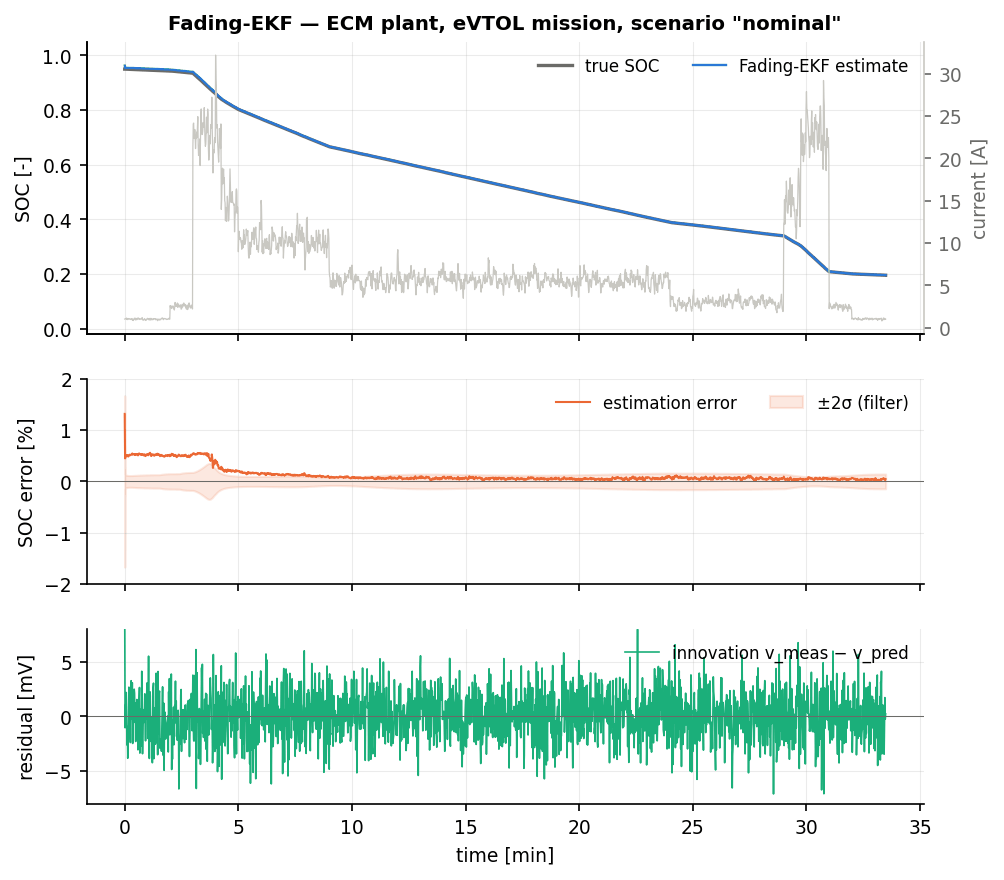
\includegraphics[width=\textwidth]{figures/cell_FadingEKF_nominal.png}
\caption{Fading-EKF on the nominal eVTOL mission: true and estimated SOC (top), estimation error with the $\pm 2\sigma$ band when available (middle), voltage residual (bottom).}
\end{figure}
\begin{figure}[H]\centering
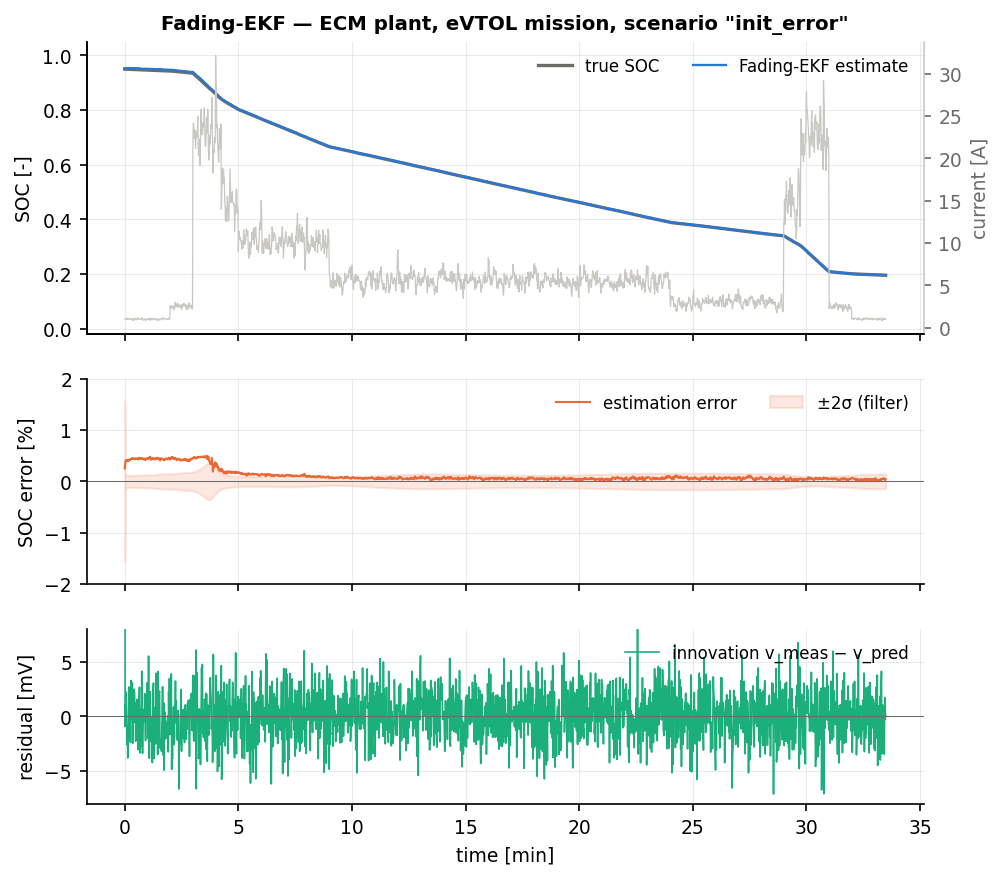
\includegraphics[width=\textwidth]{figures/cell_FadingEKF_init_error.png}
\caption{Fading-EKF with a 35\,\% initial SOC error.}
\end{figure}
\begin{figure}[H]\centering
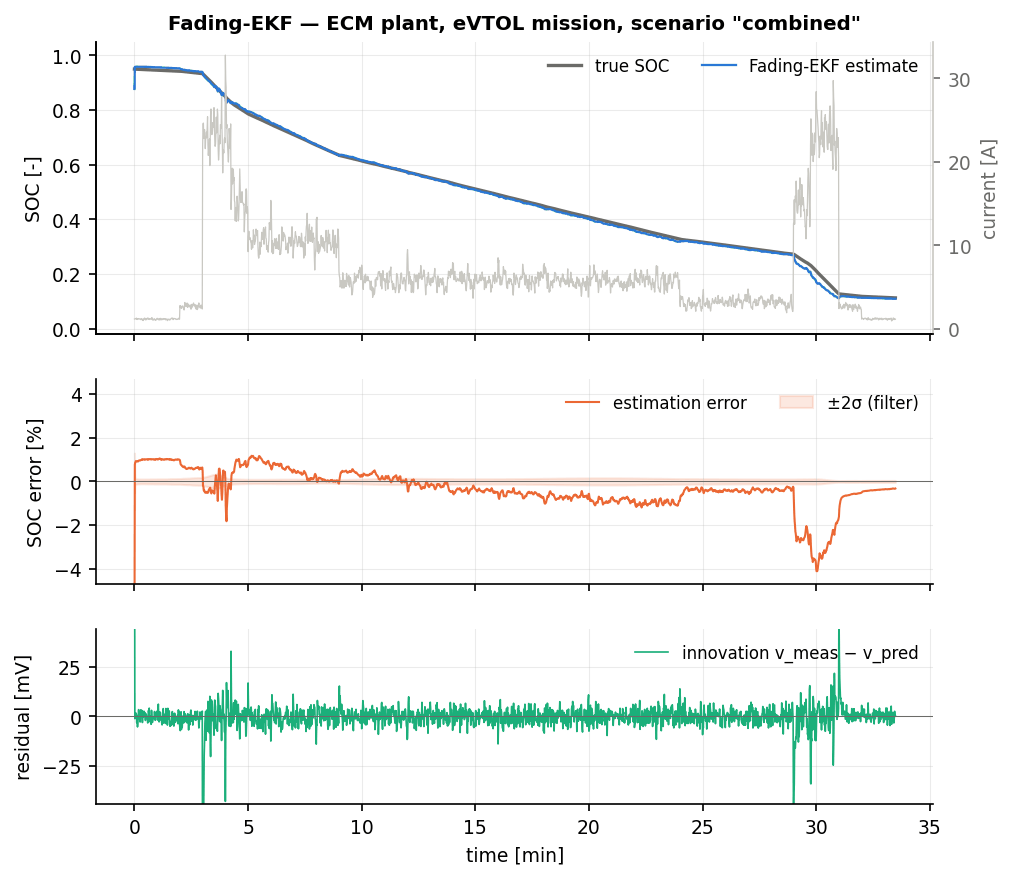
\includegraphics[width=\textwidth]{figures/cell_FadingEKF_combined.png}
\caption{Fading-EKF on the \texttt{combined} scenario (25\,\% initial SOC error, \SI{150}{\milli\ampere} current bias, 2\,\% gain error, 10\,\% capacity loss with the associated resistance growth).}
\end{figure}
\begin{figure}[H]\centering
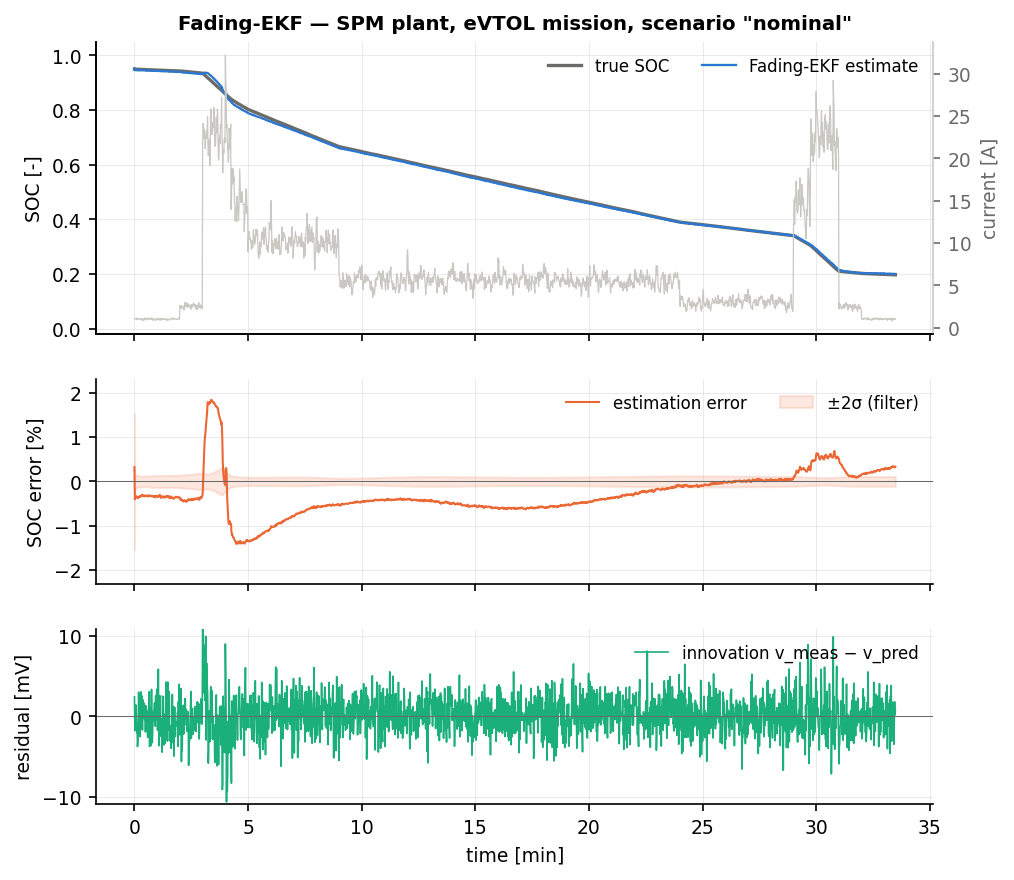
\includegraphics[width=\textwidth]{figures/cellspm_FadingEKF_nominal.png}
\caption{Fading-EKF on the electrochemical (single-particle) plant, nominal mission: the estimator uses a 2-RC ECM fitted to that plant and therefore sees a structured \SI{4}{\milli\volt} residual instead of white noise.}
\end{figure}

All figures below are three-seed means in \% SOC, as tabulated above; the plain \texttt{EKF} run on
the same data is the reference (\texttt{EKF ref.} column).  For orientation, the EKF scores
$\mathrm{rmse}_{ss}$ = 0.05\,\% on \texttt{nominal}, 0.12\,\% on \texttt{noise\_step}, 0.21\,\% on
\texttt{outliers}, 0.46\,\% on \texttt{sensor\_dropout}, 1.36\,\% on \texttt{param\_mismatch},
1.52\,\% on \texttt{aged\_cell} and 12.44\,\% on \texttt{combined} (where it never converges), and
3.73\,\% on the nominal SPM mission.

\paragraph{Benign scenarios.}  \texttt{nominal}: $\mathrm{rmse}=0.21\,\%$,
$\mathrm{rmse}_{ss}=0.05\,\%$, identical to the EKF's $0.15\,\%$ / $0.05\,\%$ in steady state and with
a \emph{smaller} maximum error ($1.02\,\%$ against $1.07\,\%$).  The six-fold larger gain predicted by
\eqref{eq:fm:gainfloor} costs nothing measurable here because the noise term is not what limits the
SOC estimate on this plant.  \texttt{init\_error}: $\mathrm{rmse}=0.18\,\%$,
$\mathrm{rmse}_{ss}=0.05\,\%$, converging at $t=\SI{0}{\second}$, again with the smallest maximum
error of the whole family ($0.59\,\%$ against the EKF's $0.62\,\%$) because the larger gain removes the
initial offset faster.

\paragraph{Target scenario \texttt{combined}.}  The Fading-EKF is the best of the eight adaptive
filters on the benchmark's hardest ECM scenario.  The EKF never converges ($t_\mathrm{conv}=$ --,
$\mathrm{rmse}=16.02\,\%$, $\mathrm{rmse}_{ss}=12.44\,\%$); the Fading-EKF converges at
$t=\SI{0}{\second}$ with $\mathrm{rmse}=\mathbf{0.93\,\%}$ and
$\mathrm{rmse}_{ss}=\mathbf{1.18\,\%}$ --- a $\mathbf{17\times}$ reduction of the full-run RMSE and a
$\mathbf{10.5\times}$ reduction of the steady-state RMSE, with the maximum error down from $29.64\,\%$
to $7.36\,\%$.  The explanation is \eqref{eq:fm:gainfloor}: the $25\,\%$ resistance growth puts a
\SI{16}{\milli\volt} bias on the predicted voltage, which the flat OCV curve near $\soc=0.9$ amplifies
into a large SOC bias of gain-dependent magnitude; a six-fold larger gain floor divides the resulting
steady-state SOC bias by roughly the same factor, and the \SI{25}{\second} memory means the
current-bias-driven drift is corrected six times faster as well.  It also keeps the best voltage
prediction of the family on this scenario after the STF ($\mathrm{rmse}_v=\SI{5.16}{\milli\volt}$,
essentially the EKF's \SI{5.15}{\milli\volt}, against \SI{14}{\milli\volt}--\SI{17}{\milli\volt} for
the $\mR$-adapting filters).

\paragraph{Other mismatch scenarios.}  \texttt{sensor\_dropout}: $\mathrm{rmse}$ $0.72\to0.21\,\%$,
$\mathrm{rmse}_{ss}$ $0.46\to0.05\,\%$ --- a $3.4\times$ / $9.2\times$ improvement and the joint best
in the family, because the filter simply forgets the \SI{15}{\second} of frozen data within a
comparable time.  \texttt{param\_mismatch}: $1.28\to1.27\,\%$ and $1.36\to1.31\,\%$, essentially a
draw.  \texttt{outliers}: $0.52\to0.25\,\%$ and $0.21\to0.09\,\%$, a useful $2.1\times$ / $2.3\times$
even though nothing in the design targets impulsive noise --- the shorter memory simply flushes each
spike out faster.

\paragraph{Where it costs.}  \texttt{aged\_cell} is worse than the EKF ($\mathrm{rmse}=1.67\,\%$,
$\mathrm{rmse}_{ss}=1.78\,\%$ against $1.18\,\%$ / $1.52\,\%$), for the same reason the STF is worse
there: the dominant error is a voltage bias, and a larger gain makes a biased measurement more
influential, not less.  \texttt{current\_bias} is also slightly worse ($0.66\,\%$ against $0.61\,\%$)
and \texttt{cold} likewise ($0.25\,\%$ against $0.16\,\%$).  The clearest regression is
\texttt{preisach}, whose numbers moved with the corrected hysteresis sign convention: $1.08\,\%$ /
$0.86\,\%$ with $t_\mathrm{conv}=\SI{224}{\second}$ against the EKF's $0.58\,\%$ / $0.20\,\%$ at
\SI{16}{\second} --- a factor of four worse, and for exactly the aged-cell reason, since an
un-modelled hysteresis voltage is an output-side error that a larger gain amplifies.
\texttt{noise\_step} costs a factor of $1.3$ in $\mathrm{rmse}_{ss}$ ($0.16\,\%$ against $0.12\,\%$)
because the permanently larger gain lets more of the \SI{20}{\milli\volt} sensor noise through ---
still an order of magnitude inside the acceptance bound, and vastly better than the STF's $2.34\,\%$
on the same scenario, because a \emph{fixed} $\alpha$ cannot be fooled by the noise into inflating
further.  That robustness of the non-adaptive design against exactly the ambiguity that defeats the
STF is worth noting: sometimes the dumber method is the safer one.

\paragraph{Cost.}  \SI{501}{\nano\second}/step against the EKF's \SI{478}{\nano\second}/step --- the
cheapest method in the whole family, with no data-dependent branches.

\paragraph{Electrochemical (SPM) plant.}  This is the Fading-EKF's best result anywhere in the
benchmark.  With the estimator running a 2-RC ECM fitted to the single-particle plant, the residual is
a structured, slowly varying \SI{4}{\milli\volt} signal produced by Butler--Volmer kinetics and a
\SI{556}{\second} diffusion time constant that two RC branches cannot follow.  The Fading-EKF ends the
nominal SPM mission at $\mathrm{rmse}_{ss}=\mathbf{0.36\,\%}$ against the EKF's $3.73\,\%$ --- a
$\mathbf{10.4\times}$ improvement, the best figure of any estimator in this family on any plant, and
against $3.02\,\%$--$3.33\,\%$ for the four $\mR$-adapting filters, which manage only $10$--$20\,\%$.
The mechanism is the whole point of the method.  Covariance matching reads the \SI{4}{\milli\volt}
residual as sensor noise, raises $\hat{\mR}$ and \emph{lowers} the gain, which hands the SOC estimate
to the coulomb integrator --- and the integrator is precisely the faulty component here, because the
fitted $Q_\mathrm{Ah}$ and coulombic efficiency do not reproduce the true lithium inventory, so the
estimate parks at a $3\,\%$ offset it can never leave.  The measurement is the trustworthy part: the
ECM's static $\ocv(\soc)$ map \emph{was} fitted to this plant, so inverting it locates SOC to a few
tenths of a percent.  Equation \eqref{eq:fm:pred} bounds the filter's memory at
$\tau=\SI{25}{\second}$ regardless of what the residuals look like, so the estimate is always
dominated by the last half-minute of voltage rather than by half an hour of accumulated model error
--- and that is exactly the right thing to do when the model, not the sensor, is the unreliable
component.  The ordering of the two families is therefore the mirror image of the ECM
\texttt{aged\_cell} row above, where the error sat in the output map and inflating $\mR$ won.  The
advantage is uniform across the SPM scenarios: \texttt{init\_error} $3.81\to0.48\,\%$,
\texttt{noise\_step} $3.30\to0.43\,\%$ ($7.7\times$, and the best SPM \texttt{noise\_step} result of
the family), \texttt{outliers} $1.99\to0.45\,\%$ ($4.4\times$), \texttt{current\_bias}
$5.69\to0.87\,\%$ ($6.5\times$), \texttt{hot} $2.16\to0.35\,\%$, \texttt{sensor\_dropout}
$5.31\to0.31\,\%$ ($17\times$), \texttt{param\_mismatch} $3.13\to1.95\,\%$.  Only SPM \texttt{cold}
resists ($3.45\,\%$ against $7.35\,\%$, still a $2.1\times$ gain but with a \SI{326}{\second}
convergence time): at \SI{-10}{\celsius} the diffusion time constant exceeds the filter's
\SI{25}{\second} memory by two orders of magnitude, and no amount of forgetting can make a 2-RC model
follow that.

\section{Summary}
One line of code, one design parameter, and the largest single improvement in this family on the
benchmark's hardest scenario: a $17\times$ reduction of SOC RMSE on \texttt{combined} and
convergence where the EKF has none.  Use a fading-memory EKF whenever slow, un-modelled bias is the
dominant error and a bounded error-rejection time constant is worth a modest permanent increase in
noise --- which describes most production BMS situations.  Choose $\alpha$ from the desired memory
length $\tau = 1/(2\ln\alpha)$ \emph{samples}, not from a textbook number: at \SI{10}{\hertz} the
usual $1.01$--$1.05$ are one to two orders of magnitude too aggressive.  Always pair it with a
covariance bound if any state direction is weakly observable --- without one, this filter reaches
NaN on the cell model in under \SI{200}{\second}.  Its single best result in this benchmark is on the electrochemical plant, where the 2-RC model
leaves a structured \SI{4}{\milli\volt} residual: $0.36\,\%$ against the EKF's $3.73\,\%$, a
$10.4\times$ gain, while every $\mR$-adapting filter manages only $10$--$20\,\%$ --- when the model
rather than the sensor is the unreliable component, shortening the filter's memory is exactly right.
Do not expect it to help when the error is instead a voltage bias (\texttt{aged\_cell},
\texttt{preisach}) or a noisier sensor: there, inflating $\mR$ rather than $\mP$ is what is needed.
